\documentclass{report}
\usepackage[utf8]{inputenc}
\usepackage{authblk}
\usepackage[block=ragged]{biblatex}
\usepackage{titlesec}
\usepackage{graphicx}

\graphicspath{ {./figures/} }
\addbibresource{references.bib}
\addbibresource{additional_references.bib}

\setlength{\parindent}{0em}
\setlength{\parskip}{1em}
\setlength{\emergencystretch}{10pt}

\setcounter{secnumdepth}{4}

\titleformat{\paragraph}
{\normalfont\normalsize\bfseries}{\theparagraph}{1em}{}
\titlespacing*{\paragraph}
{0pt}{3.25ex plus 1ex minus .2ex}{1.5ex plus .2ex}

\begin{document}
\begin{titlepage}
    \begin{center}
 
        \Huge
        \textbf{To Extract Physiology Information During Exercise using a Smartphone}
 
        \LARGE
        Mini Thesis for Probation Review
 
        \vspace{0.5cm}

        \textbf{Liqun Wu}

        \Large
        Supervised by Dr Caroline Li
 
        \vfill
 
        \vspace{0.8cm}
 
        
\includegraphics[width=0.4\textwidth]{figures/logo.jpg}
 
        \Large
        School of Computing\\
        University of Kent\\
        June 2019
 
    \end{center}
\end{titlepage}

\tableofcontents
\listoffigures

\chapter{Introduction}
\section{Aim}
The market has great demand for reliable, portable and affordable instruments that is capable for respiratory frequency measurement indoors and outdoors. This research aims deliver an alternative solution by developing a mobile application that utilises the acoustic respiration signals collected from a headset’s microphone to estimate the respiratory frequency and detect the respiratory phase in real-time. 

\section{Motivation}
In areas such as sports training monitoring and clinical monitoring, respiratory frequency is a significant measure because it contains informative indicators about athletes' performance and potential diseases. Efficient breathing approaches could contribute to athletes' performance, thus it is also essential to identify respiratory phases and analyse breathing patterns. Methods of estimating respiratory frequency widely applied include measuring the airflow of breathing, the expansion of chest wall and abdominal cavity, and the air temperature or humidity around nose \cite{Massaroni2019Contact-BasedRate}. Most of commercially available products are expensive and complicated, which are not suitable for daily-life usage. 

Being able to classify inhalation sound and exhalation sound is the foundation of estimating respiratory frequency and detecting respiratory phase. There have been many studies demonstrating that acoustic respiration signal contains enough features for being used in discriminating inhalation sound and exhalation sound \cite{Hamke2019DetectingMachines}\cite{Kaur2017UseRespiration}\cite{Ren2015Fine-grainedSmartphones}. It suggests a user-friendly, low-cost, and reliable solution to extract respiration-related information from respiration sound. 

\section{Objectives}
To investigate the feasibility of bringing a low-cost, intuitive and portable respiration monitoring solution. The major objective of this study is
\begin{itemize}
\item to design and develop a mobile-friendly solution that estimates respiratory frequency and determine respiratory phase and respiratory depth by utilising the acoustic respiration signal collected from headset’s microphone during running or resting.
\end{itemize}

It is also required to have respiratory frequency measures from other industry standard or gold standard instruments for labelling and referencing. The instruments used as comparison should not obstruct the respiratory sound collecting process, for example covering nose and month area. There are some solutions meeting our requirements, such as Equivital TnR suite which is selected as an industry standard instrument in this study \cite{equivital}. Although some work has been undertaken to validate Equivital TnR suite, it is still worthy to compare its performance against another gold standard instrument while being used in various scenarios In this case, Squark b2 from COSMED is selected \cite{cosmed}. Thus, the next objective is 
\begin{itemize}
\item to compare the difference in accuracy between Equivital TnR suite and Cosmed Squark b2 in estimating respiratory frequency while standing and running. 
\end{itemize}
\chapter{Review of Relevant Work}
\section{Respiration related knowledge}
Breathing is an essential activity for our body which allows the air exchange between the human body and the external environment. There are mainly two functions supported by the respiratory system, providing oxygen to the tissues of body and eliminate carbon dioxide from the tissues of the body. 

\subsection{Respiration in sport monitoring}

As exercise begins, the increase in lung ventilation (breathing) is directly proportional to the intensity of exercise and metabolic needs. This is shown on the adjacent chart. Note that lung ventilation is expressed as the number of air inhalations (L / min) inhaled and exhaled per minute. Increase ventilation in two ways to meet your workout needs:1. The increase in "tidal volume" refers to the amount of air inhaled and exhaled per breath. This is similar to the "wheeze amount" in the cardiovascular system.2. The increase in "breathing or respiration rate" refers to the number of times each person completes inhalation and exhalation per minute. This is similar to the "heart rate" in the cardiovascular system. If exercise is intense, the breathing rate may increase from a typical rest rate of 15 breaths per minute to 40-50 breaths per minute. The most common measure of exercise and respiratory function is called VO2 (oxygen uptake). VO2 refers to the amount of oxygen absorbed and used by the body. With continuous exercises (duration longer than 1 minute), such as aerobic fitness, longer anaerobic fitness and lesser muscle endurance training, VO2 increases linearly with increasing exercise intensity. This is because as the movement continues, more and more oxygen is relied on to help provide energy. As the intensity of exercise continues to increase, one reaches the highest point beyond which oxygen consumption does not increase further. This point is called VO2 max, as shown in the figure below. The training type has medium intensity, lasts longer (≥1 minute), and has short or no rest throughout the process, which forms the so-called "EPOC". EPOC stands for "oxygen consumption after excessive exercise" and is related to the need to keep oxygen consumption at the end of the exercise at a rate greater than the resting rate to compensate for the oxygen "debt" generated at the beginning of the exercise. We will explain more about the chart below. It may take 10-20 minutes after exercise to restore normal breathing rate through hypertrophy training.

Unlike other physiological measures, such as heart rate, blood pressure, and ECG signals, respiratory frequency is usually neglected during sports training monitoring. The study conducted by Nicolo et al suggested that respiratory frequency and physical effort has the strongest correlation compared to other physiological measures.\cite{Nicolo2017RespiratoryMeasure} The study showed that by extracting information from the respiration frequency, it is possible to analyse athletes' performance from an more advanced perspective.


\subsection{Respiration in clinical monitoring}

Two common forms for breathing includes chest breathing and abdominal breathing. One complete breath cycle includes an inhalation and an exhalation. The number of breaths per minute is called the respiratory rate. Respiratory frequency refers to the number of breaths per minute. The respiratory frequency of an adult at rest is approximately 12-18 breaths per minute and 30-40 breaths per minute for children. Adults who have a respiratory frequency of more than 20 breaths per minute may be in unhealthy conditions. A respiratory frequency of over 24 breaths per minute indicates serious health issues. It was also reported that a respiratory frequency over 27 breaths per minute is very likely to associate with cardiac arrest.\cite{Cretikos2008OfMBA} Therefore, by detecting the respiratory frequency of the athletes after training, it is beneficial to ensure their health and timely detection of abnormal physical conditions. Therefore, respiratory frequency is an indicator of some serious illnesses.

\section{Methods for respiratory frequency measurement}
Most of the solutions on the market are expensive and not suitable for everyday life, and some products are invasive, which is not available for outdoor use. The approaches widely used to measure respiratory frequency are mainly divided into two categories, one is direct measurement and the other is indirect measurement.The parameters considered in direct measurement includes respiratory airflow, respiratory sound, air temperature, air humidity and air components, chest-wall movement, cardiac activity (electrocardiography and photoplethysmography) are considered in indirect measurement. 
\cite{Massaroni2019Contact-BasedRate} 

These two types of solutions have very clear concerns. In the study completed by Massaroni, the accuracy and main advantages and disadvantages of these methods in different environments were compared. Breathing airflow-based solutions have the best performance in terms of accuracy, but they are invasive and inconvenient to use outdoors or in unstructured environments. Solutions based on air temperature, humidity and composition can provide sufficient accuracy, but are greatly affected by the environment, whether indoors or outdoors. However, solutions based on chest motion and cardiac activity can support acceptable measurements both indoors and outdoors, depending on the implementation, but if the accuracy is disturbed by motion. Respiratory sound-based solutions are also of interest to this research, providing adequate measurement performance both indoors and outdoors, but are susceptible to environmental disturbances. As the popularity of smartphones grows, more and more sports and medical-related applications appear on mobile platforms.

Of all the solutions mentioned above, only the breathing sound is the easiest to collect indoors and outdoors, because only the microphone is needed, and other parameters require additional sensors to acquire, which creates an additional barrier for measuring respiratory rate. . If it is possible to reduce noise from the surrounding environment, it is possible to expand the method based on breathing sound and improve accuracy. This is also one of the main goals of this research.


\section{Applications for extraction of respiration information}
A vast amount of studies have proven that the acoustic signals of breathing carry a lot of information about human health that can be used in classifiers to identify unhealthy people and determine the severity of the disease. In these studies, commercial headset microphones or smartphones built-in microphones. According to their experimental results, the signals collected by these devices are enough to be used to extract respiratory-related information. The researches that utilise the acoustic respiratory signal for different applications are reviewed as followed as guidelines for this study.

\subsection{Disease screening}
Stethoscopes are the most commonly used diagnostic tools for physicians to collect and amplify sounds from the heart, lungs, arteries, veins, and other internal organs. Most of this instrument is used only at the beginning of the diagnosis and does not represent the final diagnosis. The process by which the microphone collects the acoustic signal of the breath is the principle of mimicking the stethoscope.  

The respiratory sound based classifier is able to provide accurate diagnostic identification for breathing disorders, such as flu, pneumonia and bronchitis. By taking the advantage of the combination of enhanced perceptual and cepstral features, the classifier has a great potential in the diagnostic process.\cite{Lei2014Content-basedFeatures} The smartphone-based application developed by chinazunwa is able to recognise respiratory symptoms, such as cough, wheeze and stridor in real-time scenarios by using machine learning algorithms with respiratory signal.\cite{Uwaoma2017OnAlgorithms} The approach presented by Eric is an low-cost and reliable home-based alternative to clinical level spirometry which is able diagnose obstructive lung ailments in various degrees. It uses the built-in microphone to estimate the respiratory flow rate during a spirometry test.\cite{Boriello2012SpiroSmart} In addition to being able to identify diseases associated with different respiratory systems, the acoustic signals of breathing can also be used to distinguish the severity of certain diseases. In addition to being able to identify diseases related to different respiratory systems, according to Fatma, the approach that applying signal processing technique such as wavelet transforms with artificial neural networks on respiratory sound is able to classify subjects with no, mild, moderate and severe asthma.\cite{Gogus2015ClassificationNetworks} By combining the acoustic signals of breathing with other types of signals, it can identify a wider range of diseases. By utilising the combination of respiratory flow, laryngeal motion and swallowing sounds, The method proposed by Katsufumi Inoue claiming to achieve 86.0\% specificity and 82.4\% sensitivity on identifying patients with dysphagia.\cite{Oku2018UsingSwallowing}


\subsection{Clinical monitoring}
Application software using respiratory acoustic signals has a more diverse use scene in the field of Clinical monitoring. The system proposed by jinglong niu is able to detect the presence of sputum in a patient’s trachea especially for the intubated subjects by analysing their respiratory sound. It is able to reduce the cost of medical staff since they must check the respiratory state periodically to prevent sputum deposition which could block the airways of patients and cause severe consequence.\cite{Niu2019AState} It shows the value of continuous monitoring when the clinical monitoring is limited and expensive. 
Besides, the system StressSense developed by Hong detects human stress level both in indoor and outdoor environments based on the human voice collected from the microphone embedded in mobile phones. It provides a relatively reliable and non-invasive monitoring solution for detecting stress in real-life situations.\cite{Lu2012StressSense:Smartphones}

The environment for monitoring the patient's sleep quality is relatively strict, and the patient is required to sleep in the ward for one night, during which various physiological indicators are measured. Because of the different sleeping environments, this measurement may not represent the patient's actual sleep quality. It is, therefore, valuable to be able to monitor the quality of sleep in the home. Use smartphone’s microphone to estimate respiratory frequency to determine patients’ sleep quality which provides an cheap and accessible alternative to polysomnography test.\cite{Kaur2017UseRespiration} Unlike most of the sleep quality monitoring applications only focus on detecting body movement, cough and snore, the system proposed by yanzhi aims for providing fine-grained sleep monitoring by leveraging smartphones for collecting respiratory sound. The system not only detects snore, cough, turn over and get up also provide respiratory frequency based on acoustic features extracted from the respiratory sound.\cite{Ren2015Fine-grainedSmartphones}

Fine breathing-related information can help to better understand the patient's breathing patterns and methods. As an alternative to airflow based respiratory phase detection, the approach proposed by omar claims to achieve to 95\% accuracy in distinguishing inspiration and expiration phases using the acoustic respiratory sound signal collected from the microphone placed in front of subject’s nose.\cite{Yahya2014AutomaticCycles} Moreover, Eric developed an unsupervised machine learning approach to process respiratory sound to predict fine respiratory parameters respiratory depth or length by using linear predictive coefficients and restricted boltzmann machines. \cite{Hamke2019DetectingMachines}

A system claimed to be capable of detecting the respiratory frequency indoors using the acoustic respiration signals collected by the headset’s microphone and achieves high accuracy in estimating respiratory frequency at both low and high respiratory frequencies.\cite{Nam2016EstimationHeadset} However, the subjects did not breathe naturally in the experiment, but breathed at a fixed frequency under the instruction of the researchers. The breathing sound collected might be exaggerated because of the unnatural breathing approach. Moreover, most people do not breathe at a constant respiratory frequency. Nonetheless, this result still shows that the acoustic respiration signal includes sufficient features that can be used to estimate the respiratory frequency. Also, there are some methods of indirect measurements, such as a non-invasive approach that takes advantage of the fusion of multiple physiological measures to infer the waveform of respiration to achieve detecting respiratory frequency.\cite{Mason2002SignalMonitoring} However, it is still challenging to collect multiple physiological measures at the same time outdoors.


\chapter{Research Description}
\section{Introduction}
The ultimate goal of this research is to develop a mobile application to estimate respiratory frequency based on the respiratory sound signal collected from a headset's microphone. Various signal processing methods and machine learning models will be experimented to achieve the objectives. The approaches designed and some potential contribution are discussed in the following sections.

\section{Approaches}
To provide the estimation in respiratory frequency, it is fundamentally necessary to be able to discriminate inhalation sound and exhalation sound from the breathing sound collected. Once it is capable of identifying the category of the breathing sound,  respiratory rate can be calculated accordingly. Fine respiratory information, such as respiratory depth and respiratory phase can also be provided.

It is getting more and more popular to classify audio clips based on the spectrograms generated using convolutional neural networks. Instead of hand-crafting features, convolutional neural networks are expected to find useful features automatically during training with no supervision required. Also there have been many pre-trained models available for the purpose of transfer learning. Therefore, various convolutional neural networks are going to be modified and experimented. In order to generate spectrograms that capture valuable features, a number of pre-processing and frequency-time based signal processing methods will be tested in order to improve the performance of the classifiers. Apart from exploring the performance of convolutional neural networks, other machine learning models like Support Vector Machine and Random Forest are of interest. various temporal and spectral features will be evaluated in this approach. 

The working solution will finally be implemented for mobile platform with computational efficiency considered. Since the computational resources in mobile platform are restricted, It is expected to make adjustments to balance the performance for real life using.

\subsection{Experimental design}

\subsubsection{Participants and eligibility criteria}
20 healthy males/females aged 18-45 will be recruited. Subjects with pulmonary, cardiovascular or metabolic disease, injuries and those unable to perform the required exercises will be excluded. Pregnant women will also be excluded. An informed, written consent form will be read, understood and signed by participants before any testing. 

\subsection{Experimental series}
The purpose is to collect respiratory sound signals at different frequencies while standing still and running. The entire experiment will be carried out in the laboratory. The experiment includes two series. The subjects are required to perform Series 1 with COSMED Squark b2, Equivital TnR suite and a headset. While only Equivital TnR suite and a headset are required for the subjects in Series 2. The device required will record data throughout the two series. The two series will carry out the same experimental steps as follows. There will be a 30 minutes gap between series 1 and series 2 for the subjects to rest.

\begin{enumerate}
\item Stand still and breathe naturally for five minutes.
\item Warm up for 3 minutes on the treadmill at 8km/h.
\item Increase the speed for male and female subjects to 10.8km/h and 9km/h and keep running for 3 minutes.
\item Increase the speed for male and female subjects to 12.6km/h and 10.8km/h and keep running for 3 minutes.
\item Increase the speed for male and female subjects to 14.4km/h and 12.6km/h and keep running for 3 minutes.
\item Increase the speed for male and female subjects to 16.2km/h and 14.4km/h and keep running for 3 minutes.
\item Stop running and rest on the treadmill for 10 minutes.
\end{enumerate}

\section{Expected results}
This study is expected to find the difference in accuracy between Equivital TnR suite and COSMED Squark b2 in measuring respiratory frequency while running and standing still, and in measuring respiratory frequency while standing still and breathing at various frequencies. Also, the signals collected from the commercially available product and the gold standard tool can be used as references to verify the validity of the developed application. The study plans to develop a mobile application that estimates the respiratory frequency and detects the respiratory phase and respiratory depth, by applying the signal processing and machine learning techniques to the acoustic respiration signals collected by the headset’s microphone. The application provides reliable results when the user is standing still and running, whether indoors or outdoors.

\section{Potential contributions}
This study will propose an algorithm with founded features that is sufficient in classifying the different categories of respiratory sound. These anticipated findings can help us understand and design a user-friendly, low cost, and portable solution for daily monitoring of respiratory frequency. Respiration frequency monitoring will become accessible to more people for various purposes. 

As mentioned previously, respiratory frequency reflects a lot of valuable information of athletes’ behaviour during training, especially physical effort which is just recently discovered. The application developed in this research will also dramatically advance the existing form of sports training and help us better understand the performance of athletes. Since respiratory frequency is a indication of various kinds of diseases, the application is also expected to discover some potential health issues by providing continuous breathing monitoring in daily life. 
\chapter{Description and Evaluation of Current Work}
\section{Introduction}
The work has completed up to this stage including composing the ethics proposal for data collection and developing a system on a cloud platform for the feasibility test on the mock dataset created for temporary use. The experiment consisting of two series were introduced in the ethics proposal as the guideline for data collection in next phase. Initial experimenting work on exploring potential signal processing combinations, useful features and classifiers has been carried out. The tools, approaches applied and results obtained for the current stage are shown and evaluated in this chapter.

\section{System architecture}
The system architecture consisted of three major parts as shown in Fig. \ref{fig:system_architecture}. Data preparation and pre-processing were included in the first part. The pre-processed data was then passed to the second part of the system for feature extraction to obtain the essence of the signal. The last part of the system was responsible for two jobs, classification and estimation. The classifier discriminated segmentations based on the feature extracted and then estimated respiration related information such as respiratory frequency, respiratory phase, and respiratory depth. 

\begin{figure}[h]
    \centerline{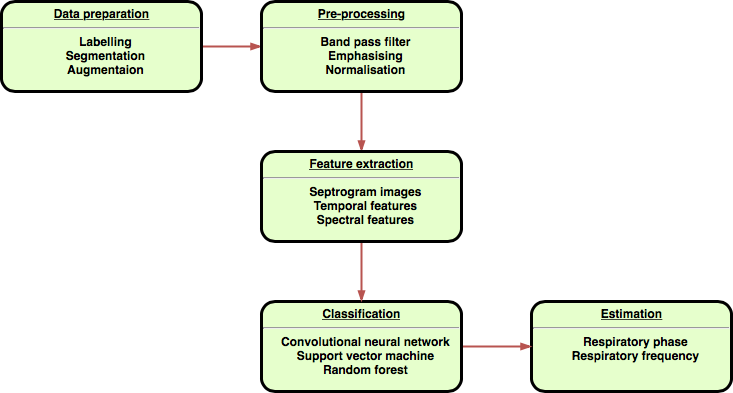
\includegraphics[scale=0.55]{figures/system_architecture.png}}
    \caption{A diagram of the system architecture}
    \label{fig:system_architecture}
\end{figure}

\section{Environment setup}
Instead of developing the system directly for the mobile platform at the initial stage, the experiment was carried out on Colaboratory. Colaboratory is an cloud Jupyter Notebook environment and ideally for fast-prototyping. The experiment programs are written in Python which is widely used in machine learning and deep learning community. Test data was stored on Google drive which is then connected to the Jupyter notebook created on Colaboratory. This approach made the file importing and exporting effortless and reliable in the experimenting process. 

There were also a number of Python libraries considered in this experiment for various purposes. Librosa is a Python library focused on audio signal processing, it implements most of the popular signal processing approaches and enables easy access to the frequently-used features in temporal and spectral analysis. PyHHT and PyWT were also tested for the implementation of Hilbert Huang Transform and Wavelet Transform, respectively. Matplotlib was selected to achieve visualisation and plots exporting. 

\section{Dataset preparation}
Prior to receiving the approval for the ethics application, a mock dataset was temporarily created from the author during a short running outdoors. The mock dataset consisted of 4 audio files in WAV format which were recorded in 22050Hz with the iOS application named Audio Memos using IPhone 6 and the microphone in the original earpods. The duration of the audio clips varies from 23 to 59 seconds.

The exhalation and inspiration segmentation contained in the dataset were manually labelled.An example of the test data with respiration phase labels is illustrated in Fig. \ref{fig:audio_waveform}. However, the markers in yellow and red only represent when the inhalation and exhalation approximately begin. A more precised and completed labelling could be obtained after the actual data collection.

\begin{figure}[h]
    \centerline{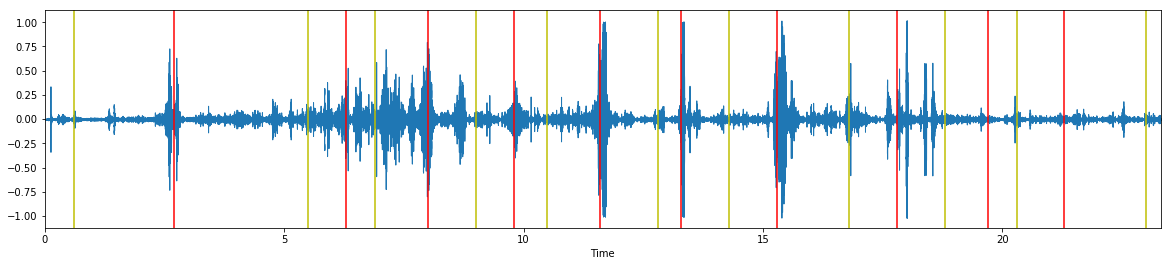
\includegraphics[scale=0.35]{figures/audio_waveform.png}}
    \caption{An illustration of a respiratory sound signal with manual labelling. Inhalation starts at yellow markers. Exhalation starts at red markers.}
    \label{fig:audio_waveform}
\end{figure}

\clearpage
\section{Signal processing methods}
The complete pre-processing pipeline consisted of 4 steps which were a band-pass filter, an emphasis filtering, normalisation and segmentation. The design of the combination of signal processing methods were inspired by \cite{Lei2014Content-basedFeatures}\cite{Niu2019AState}\cite{Ren2015Fine-grainedSmartphones}. The completed results after applying the full pre-processing techniques is shown in Fig. \ref{fig:fft_pipeline}.
\begin{figure}[h]
    \centerline{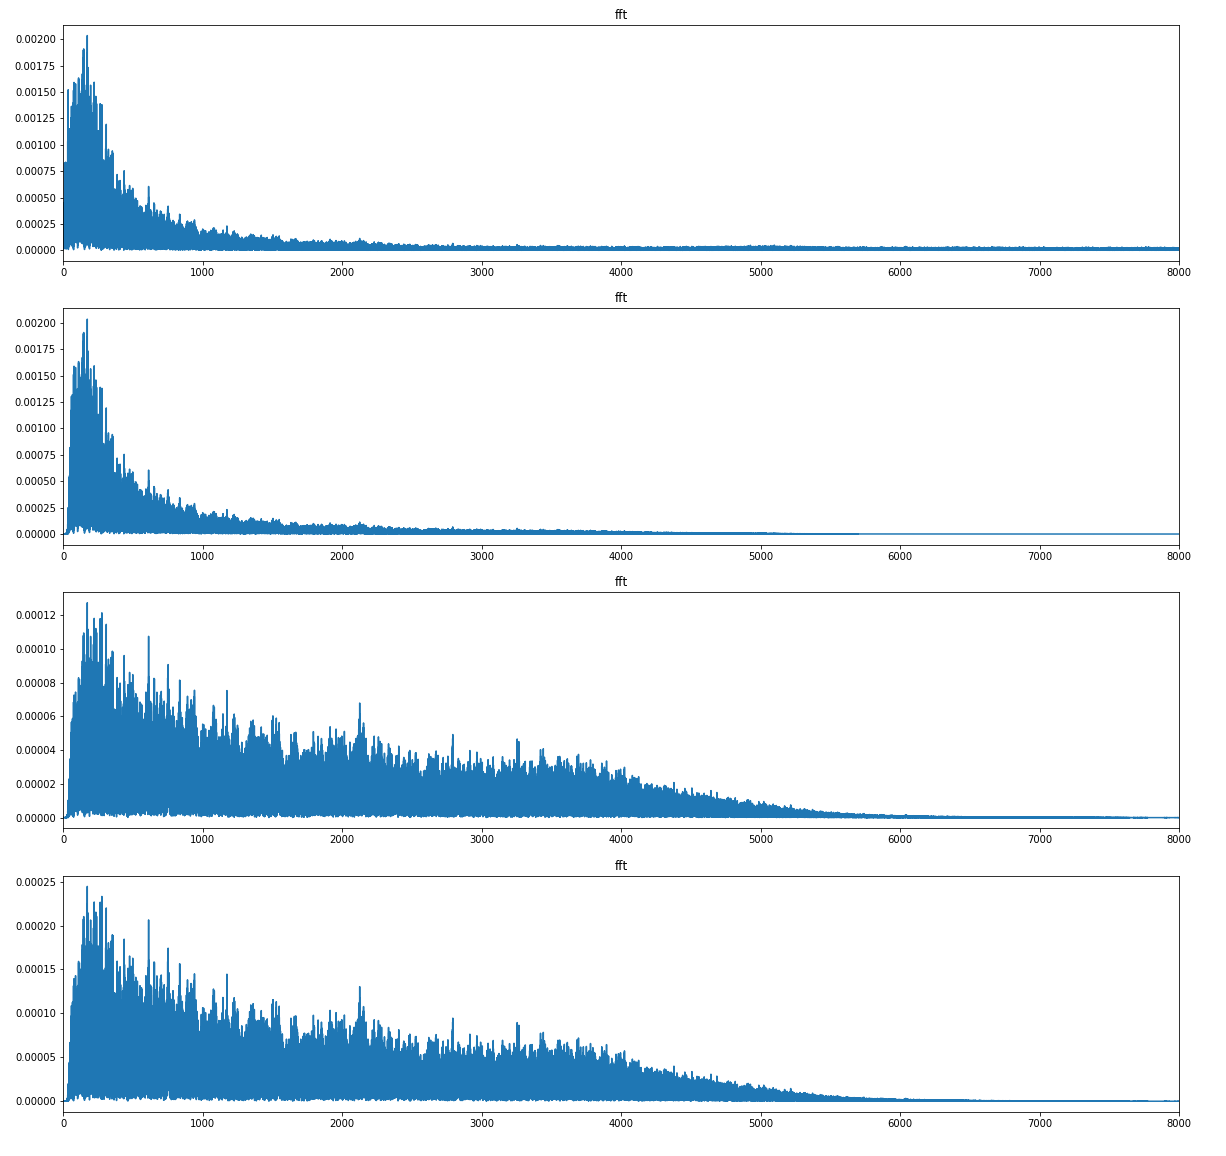
\includegraphics[scale=0.33]{figures/fft_pipeline.png}}
    \caption{The results of applying the complete signal processing methods.}
    \label{fig:fft_pipeline}
\end{figure}

\subsection{Band-pass filter}
The frequency components that contained in the four audio clips were  examined by applying Fast Fourier Transform (FFT) as shown in Fig. \ref{fig:fft}. It was clearly shown that the major frequency components were in the range of 0-2000Hz. To filter out the rest unwanted frequency, the signal data was firstly fed into a band-pass filter to retain the frequency component between 50Hz and 4000Hz. 

\begin{figure}[h]
    \centerline{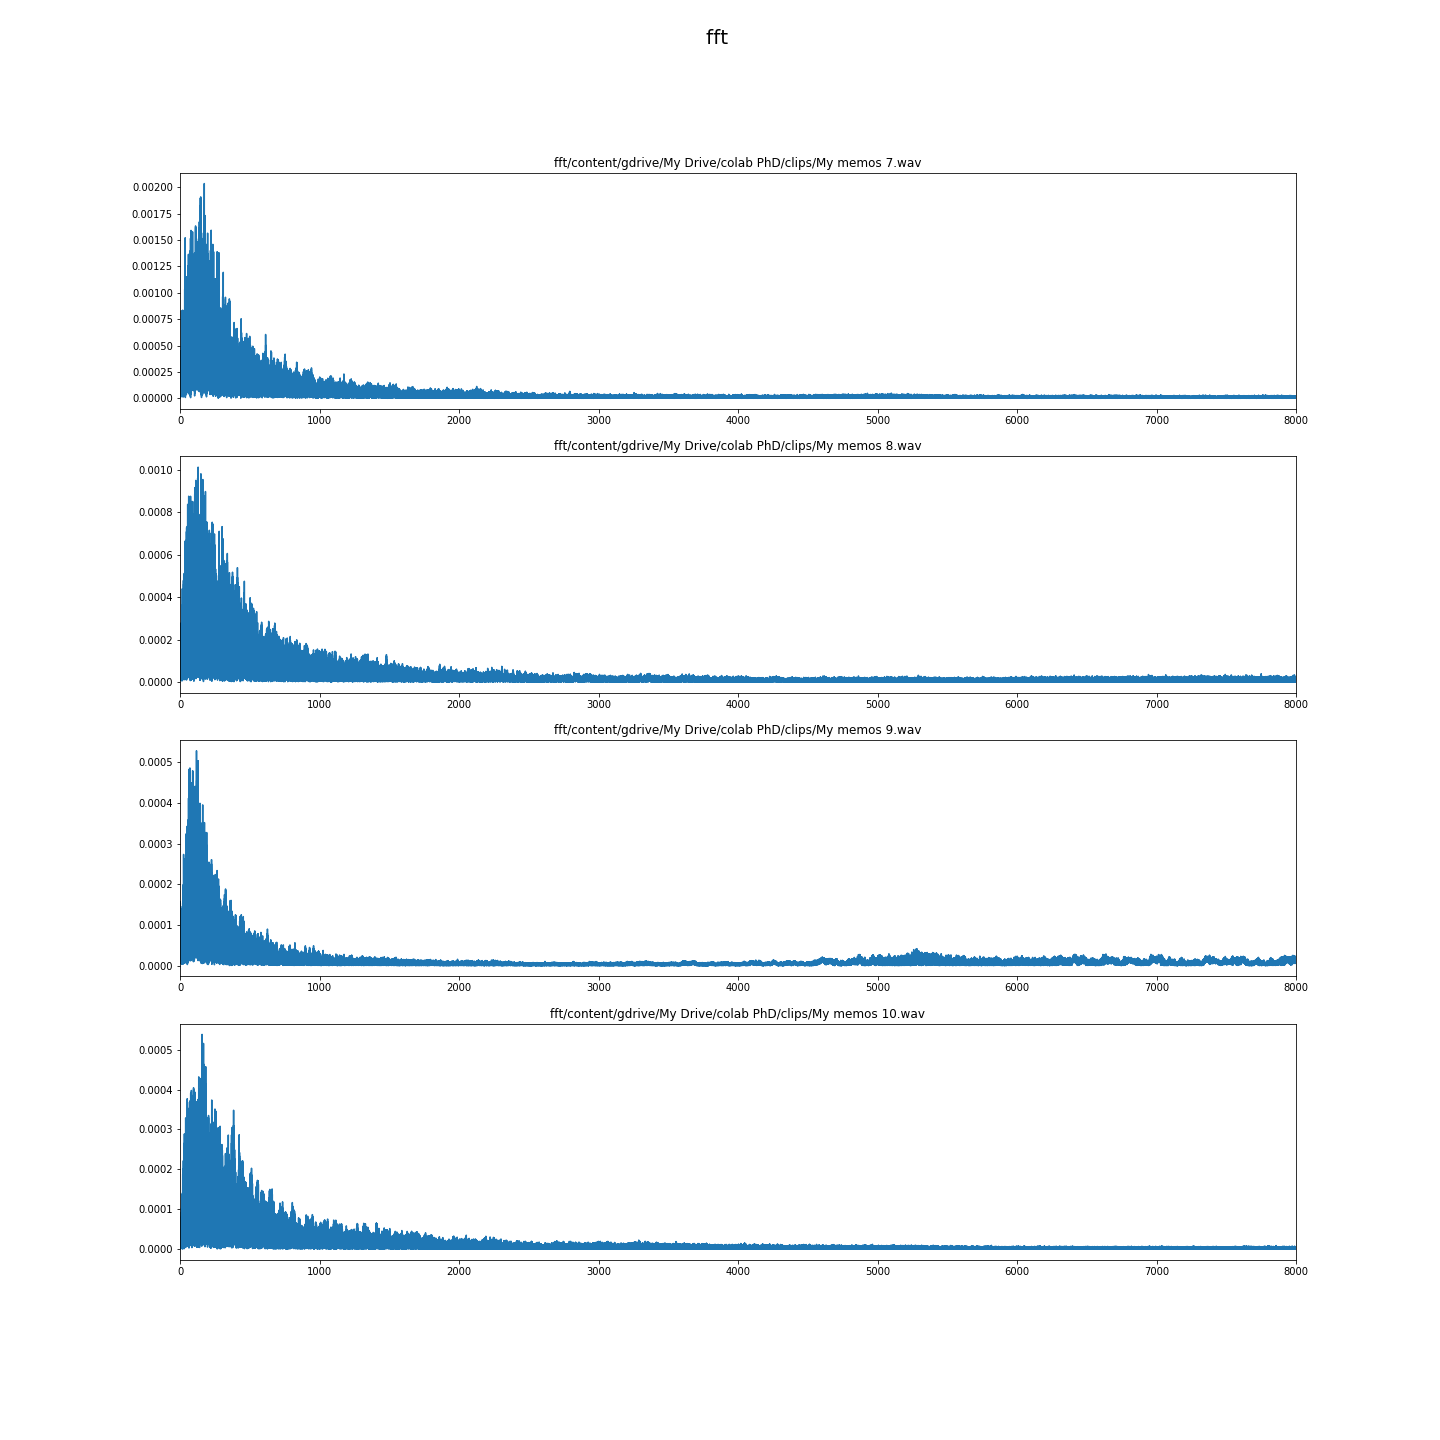
\includegraphics[scale=0.33]{figures/fft.png}}
    \caption{Frequency components of four respiratory sound signals decomposed using FFT}
    \label{fig:fft}
\end{figure}

\subsection{Emphasis filter}
To overcome the radiation effects caused mostly by the lips, the signals were applied with a pre-emphasised filter to increase the amplitude of the frequency components in high frequency range. This step is achieved by following 
\begin{equation}
s^\prime (i)=s(i) - 0.96 \times s(i-1), \qquad i=1, \ldots, N-1
\end{equation}
where $s(i)$ is the i-th sample data in the signal and $s^\prime(0) = s(0)$ when $i=0$.

\subsection{Normalisation}
Due to the variations of the devices used and the location the signals collected from, it is suggested to normalise the signal to have a stable performance.
\begin{equation}
s^\prime (i)=\frac{s(i)}{\max(|s(i)|)}
\end{equation}

\subsection{Segmentation}
Segmentations are 1000ms long having 22050 signal data points and 25\% overlapping. Hamming window is applied to segmentations to avoid spectral leakage effect. It is worth noting that segmentations created for training were likely to include some of the non-respiration sound because of the subjective labelling. Therefore, it should affect the performance of the classifier described below. 

\section{Feature extraction}
This research aims to explore the most suitable representation of spectrograms and spectral and temporal features. The results of feature extraction obtained are evaluated in the following sections. 

\subsection{Spectral features}
As illustrated in last section, FFT is great for decomposing the frequency components included in the signals. However, it only demonstrate very little information regarding the relationship between time and frequency. In order to extract the correlation between time and frequency in the signal, a number of frequency domain-based analysing approaches were evaluated, such as Short Time Fourier Transform (STFT), Wavelet Transform (WT) and Hilbert Huang Transform (HHT).

STFT provides time-frequency information by applying FFT on the window with fixed length sliding across entire signals. The spectrograms generated by STFT is then converted to mel-scaled spectrograms. Mel-scale is more ideal for representing human sound in frequency due to the fact that the non-linear perception of humans' hearing to different frequency. The comparison between STFT generated spectrogram and its mel-scaled spectrogram is shown in Figure \ref{fig:stft_mel-stft}. The mel-scaled spectrogram provides a more intuitive visualisation for exhalation than the original spectrogram. It clearly shows that most of the red markers perfectly align with one of the peaks in the spectrogram. The red markers which do not associate with any peaks were also hard to distinguish during labelling. On the other hand, it is relatively impossible to recognise the inhalation by simply looking at the mel-scaled spectrogram. 

\begin{figure}[h]
    \centerline{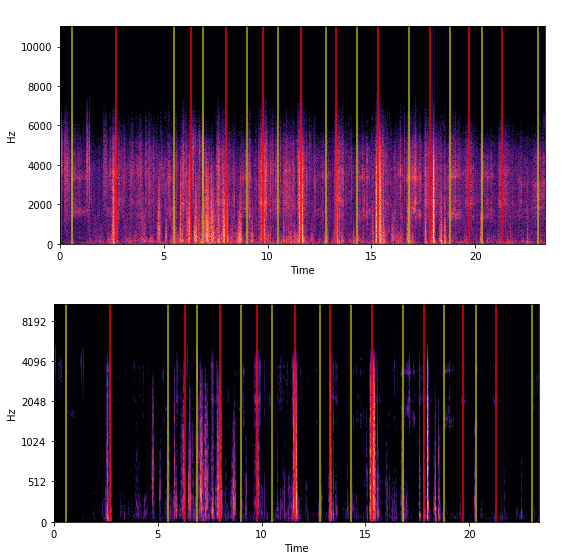
\includegraphics[scale=0.55]{figures/stft_mel-stft.png}}
    \caption{The spectrograms obtained from using STFT (top plot) and mel-scaled STFT (bottom plot). Inhalation starts at yellow markers. Exhalation starts at red markers.}
    \label{fig:stft_mel-stft}
\end{figure}

STFT has same resolution across different frequency range which is not a ideal approach for non-stationary signals with fast transient features. In contrast, WT offers good resolution in time and relatively weak resolution in frequency in high frequency range while good resolution in frequency and relatively weak resolution time in low frequency range. It would be helpful to capture the transients features by adopting continuous wavelet transform. Different wavelet functions influences the results of spectrogram generated. There were three kinds (Gaus, Mexh and Morl) of continuous wavelet function experimented as the basis functionand the results are shown in Fig. \ref{fig:wavelet_functions}. It is fairly difficult to identify which wavelet function gives the best results in representing the signal.

\begin{figure}[h]
    \centerline{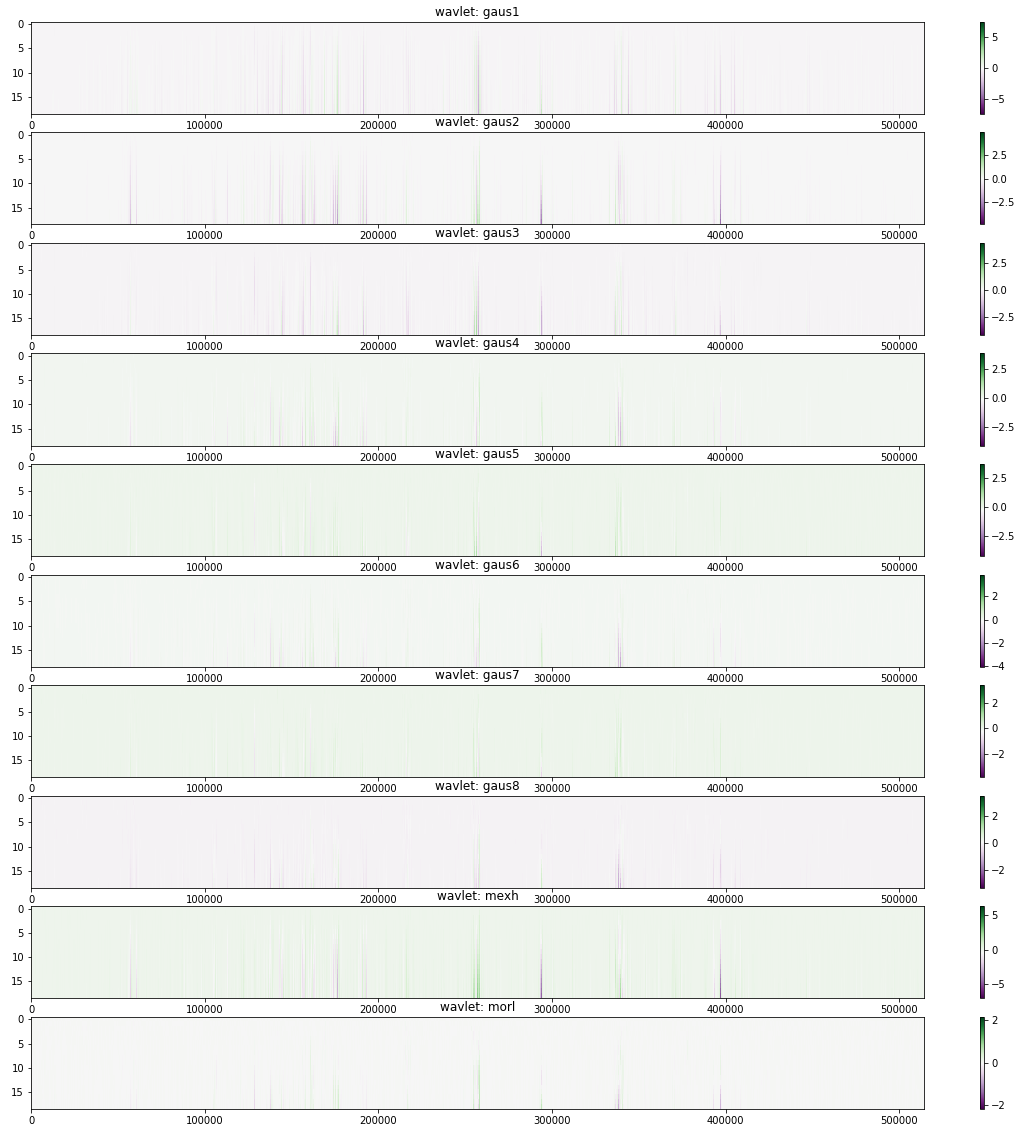
\includegraphics[scale=0.45]{figures/wavelet_trans_wav_func.png}}
    \caption{The result of applying different wavelet functions to a respiratory sound signal}
    \label{fig:wavelet_functions}
\end{figure}

\clearpage
\subsection{Temporal features}
The energy of an individual segmentation is the only temporal feature which has been implemented and evaluated so far. The energy of a segmentation is define as 
\begin{equation}
e(i) = \sum_{i=0}^{N-1}{s(i)^2}
\end{equation}

where N is the size of a segmentation and $s(i)$ is the i-th data point in a segmentation.

The purpose of using energy is to discriminate voiced and unvoiced segmentations. It could significantly reduce time spent in computation by disregarding the unvoiced segmentation in classification. This audio signal is 23s long containing 2678 segmentations as shown in Fig. \ref{fig:energy}. By setting energy threshold to the mean of the energy across the signals, only 309 segmentations were retained which still include around 90\% of the inhalation and exhalation segmentations. Therefore, segmentation energy is an effective feature in screening voiced and unvoiced segmentation. 

\begin{figure}[h]
    \centerline{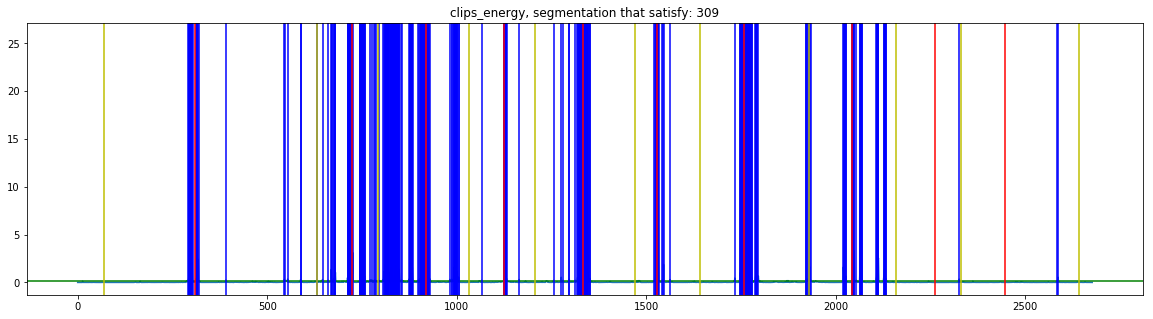
\includegraphics[scale=0.35]{figures/energy.png}}
    \caption{The blue line on the top plot represents the segmentation energy for all segmentations of a respiratory sound signal. The navy colour markers on the bottom plot correspond to the segmentations having higher energy than the energy threshold.}
    \label{fig:energy}
\end{figure}

\section{Data representation}
In order to generate training data for CNN, the spectrograms of the signals which represent inhalation and exhalation will be generated and saved in corresponding folders on the Google drive for easy access from Colaboratory. In total, there were 51 inhalation segmentations and 54 exhalation segmentations created from four respiration sound files. 20\% of the segmentation were randomly selected and then used as valid data. Partial mock dataset is shown in Fig. \ref{fig:dataset}

\begin{figure}[h]
    \centerline{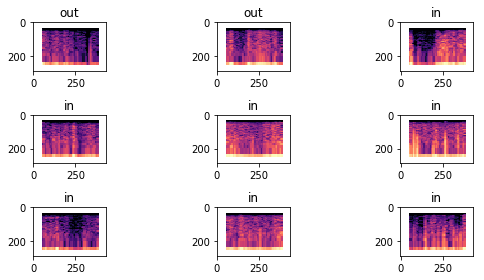
\includegraphics[scale=0.8]{figures/dataset.png}}
    \caption{Partial dataset (Spectrograms titled as 'in' represents an inhalation data. Spectrograms titled as 'out' represents an exhalation data.}
    \label{fig:dataset}
\end{figure}

\section{Classification}
Being able to correctly discriminate the sound of inhalation and exhalation is the foundation of providing respiration-related information such respiratory phase and depth. To quickly explore the feasibility of classifying respiration sound using audio signal generated spectrograms, FastAI was selected for implementation. FastAI is a high-level deep learning framework enables fast and easy process in deep learning model training and analysing. 

Transfer learning allows taking advantage of past experience from previous training. FastAI provides pre-trained models for transfer learning without developing and training a neural network from scratch. ResNet34 is a variation of convolutional neural network was used in this phase \cite{He2016DeepRecognition}.

The performance of the training phase was evaluated through three characteristics training loss, valid loss and accuracy. The model was trained for 10 epochs and the final accuracy achieved over the validation dataset was 66\%. Even the loss on the training dataset decreased over the epochs but it was significantly higher than the loss on the validation dataset. It was likely to be a sign of underfitting which suggested that the model didn't learn enough characteristics for classification from the mock dataset prepared. It might also imply that the classification model is not ideal for respiration data. However, the classification results were obtained without fine-tuning. Approaches used to improve classifier's performance is described in the next chapter. 
\begin{figure}[h]
    \centering
    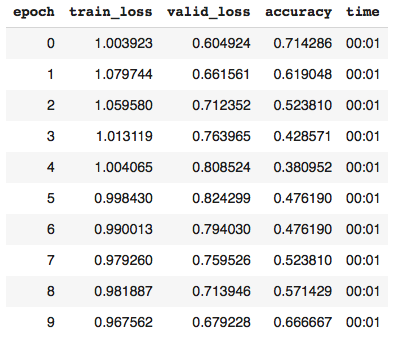
\includegraphics[scale=0.6]{figures/classification_results.png}
    \caption{Results after ten epochs training.}
    \label{fig:classification_results}
\end{figure}
\chapter{Summary and Future Research Plan}
\section{Summary}
So far, after a large number of relevant research literatures have been evaluated and the analytical methods used in the relevant studies have been considered, this study decided to use the spectrogram generated by the respiratory sound signal to estimate the frequency of breathing with CNN, to determine the stage of breathing and The depth of breathing. The work currently done includes the development of ethics proposal, the collection and labelling of test data, and the use of Colaboratory for prototyping of different signal processing, dataset generation and classifier processes. The results of the tests show that the data sets generated by manual annotation are sufficient for training of classification, and the various methods used in the signal processing flow are very effective. The signal processing flow preserves the respiratory-related frequency components while removing unwanted frequency components. Finally, through the transfer learning, using the Resent model provided by Fastai to distinguish whether a sound is an exhalation sound or an inhalation sound. The performance of the classifier trained with the test data achieved over 50\% accuracy without any fine tuning. After being able to judge the breathing phase, the frequency of breathing can be estimated accordingly.
\section{Future research plan}
Future research work focuses on preparing data, comparing other combinations of signal processing methods, and various machine learning, such as support vecter machine. The details of each of the focuses is discussed in the follow sections.
\subsection{Dataset generation}

labelling where the in/out starts by aligning the audio signal with the reference signal

Conventional data augmentation includes scaling, stratching, cropping and etc. However, the data augmentation for audio-generated spectrogram image uses completely different mechanisims.

\subsection{Signal pre-processing}
segmentation size


Hilbert huang transform

explore different combination of signal processing approach

\subsection{Feature extraction}
Excepting  

ddiscriminating the respiratory phase 

LPC feature

perceptual feature (Per)

cepstral (Cep) features

perceptual and cepstral (PerCep) features 

enhanced hybrid perceptual and cepstral (PerCepD) features.

spectural bandwidth
spectral rolloff
spectral centriod
spectral contrast
spectral flatness
spectral mfcc
spectral mfcc delta
spectral mfcc delta of delta

\subsection{Data augmentation}
The purpose of data augmentation is to increase the variety of the dataset especially when the dataset is small. Unlikely traditional image augmentation, cropping, zooming and scaling do not work well and even creating data with misleading labels. 

Data augmentation has not yet been implemented in this work. However, some research has been done in exploring approaches creating additional data based on existing dataset.\cite{Cho2017DeepBreathSettings} \cite{Schluter2015ExploringNetworks}

According to the study undertaken by Schluter and Grill, the most effective augmentation approach is pitch shifting. By also combining the time stretching and random frequency filtering, it could reduced the error signifcantly between 10 and 30\%.\cite{Schluter2015ExploringNetworks}

\subsection{Classification}
continue to use CNN when formal data is collected
experiment other machine learning for performance comparasion

SVN

random forest and support vector machine

information gain
combination of different features


\subsection{Mobile application development}

The model created and trained with Fastai will then be exported to Core ML which is a machine learning suite provided by Apple.

To transfer the complete solution to mobile platform where the computation resource is limited. 

CNN image grey scale
CNN levels

High sampling rate results in large audio files which requires a lot of computing resource 


It is necessary to explore 

aim to provide respiration-related information in real-time. therefore data size and computational complexity and time taken should be taken into account.

It might require some optimisation for fulfil the requirements. either reduce the size of the data used to represent or reduce the number of layers

also try embedded model (weighted model)

\addcontentsline{toc}{chapter}{Bibliography}
\printbibliography
\end{document}
